\section{Experimentación General}


\subsection{Comparando con el Exacto}

\quad Vamos a comparar todas nuestras implementaciones y a calcular las distancias con respecto al algoritmo exacto. Debido al costo del exacto se realizaron tests de 5 nodos a 16 con 50 repeticiones para cada cantidad. Definimos distancia como la diferencia entre el resultado exacto y el de la heurística correspondiente. Esto nos da una idea de \textit{que tan mala es la heurística}.


\quad Comparamos primero con grafos generados aleatoriamente, luego con grafos estrellas no uniformes y grafos \textit{web}.


\begin{figure}[H]
	\centering
	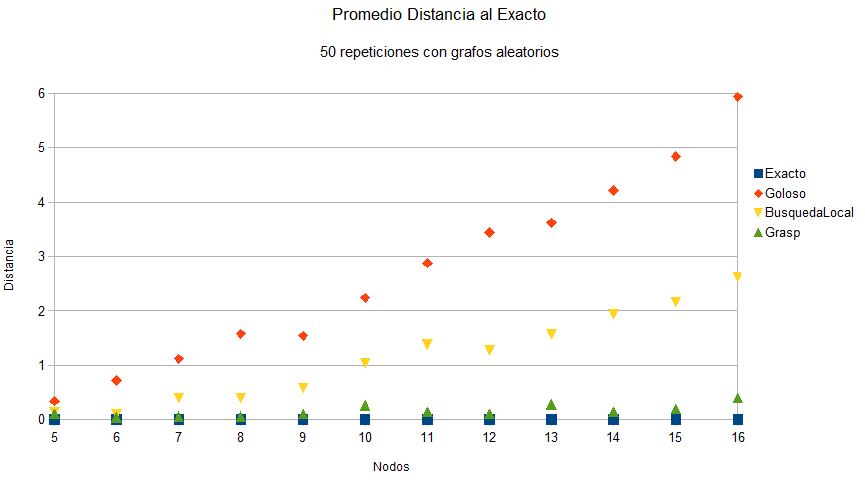
\includegraphics[scale=0.6]{distancia-Azar.png}
\end{figure}

\begin{figure}[H]
	\centering
	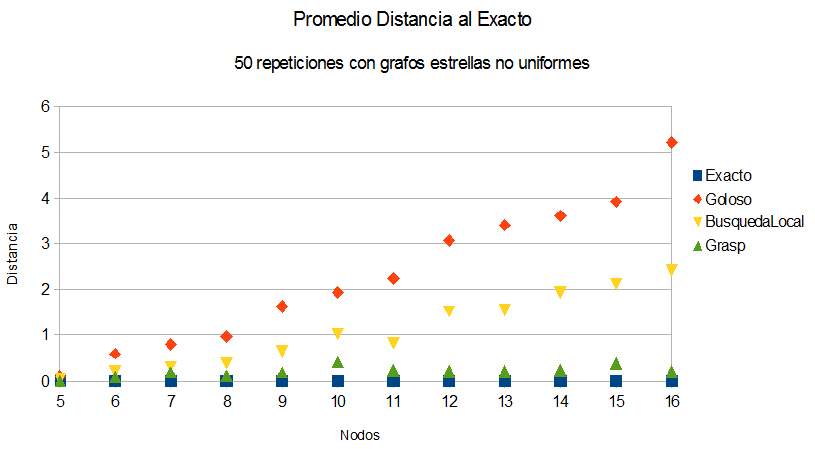
\includegraphics[scale=0.6]{distancia-Star.png}
\end{figure}

\begin{figure}[H]
	\centering
	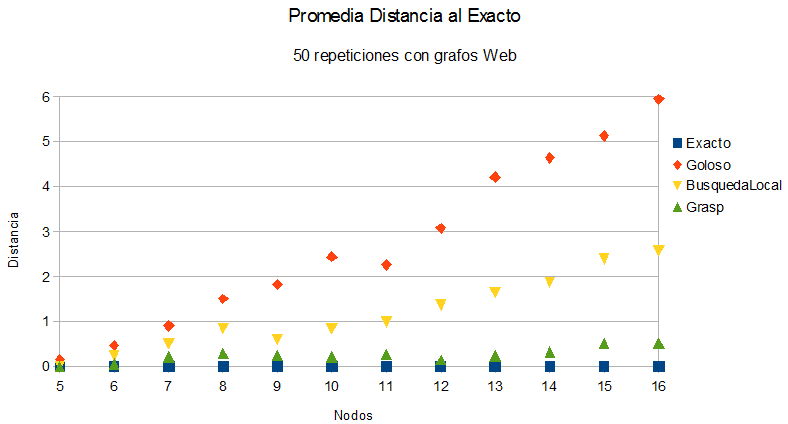
\includegraphics[scale=0.6]{distancia-Web.png}
\end{figure}

\quad Se ve claro como a medida de que se incrementan los nodos en los grafos la calidad de las soluciones obtenidas empeoran.

\quad Con respecto a la heuristica golosa es la peor de las heuristicas, sin embargo como se vera más adelante es la de menor costo temporal. El empeoramiento (distancia) es lineal a la solución exacta en las 3 familias de grafos.

\quad Con la búsqueda local pasa algo similar salvo que por los datos obtenidos podriamos decir que es prácticamente la mitad de peor que el goloso. 

\quad En cambio, con la metaheurística GRASP se obtiene distancias casi nulas con respecto a la solución exacta. Siendo en promedio menor a una para este rango de nodos de grafos que experimentamos (en las 3 familias).

\quad

\quad Ahora vamos a mostrar los datos anteriores pero comparando cada heuristica consigo misma fijándonos la distancia con la solución exacta.

\begin{figure}[H]
	\centering
	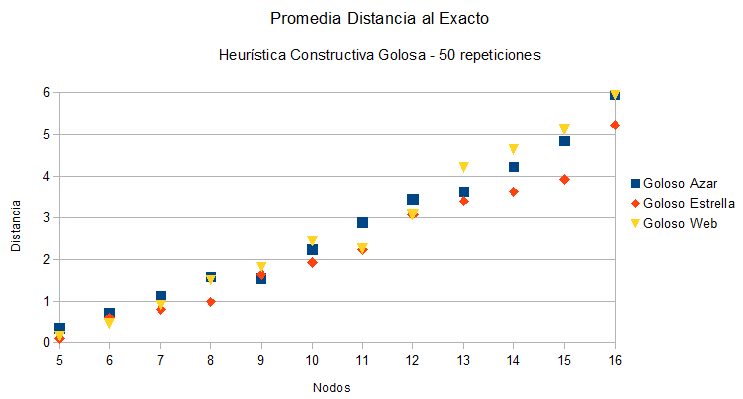
\includegraphics[scale=0.6]{distancia-Goloso.png}
\end{figure}

\quad Prácticamente el goloso se comporta igual con los tres tipos de grafos, es decir, que la calidad de las soluciones obtenidas no depende de estas familias de grafos. Podemos determinar que a pesar de la similitud, esta heurística es levemente peor con los grafos Web de 4 vértices.

\quad

\begin{figure}[H]
	\centering
	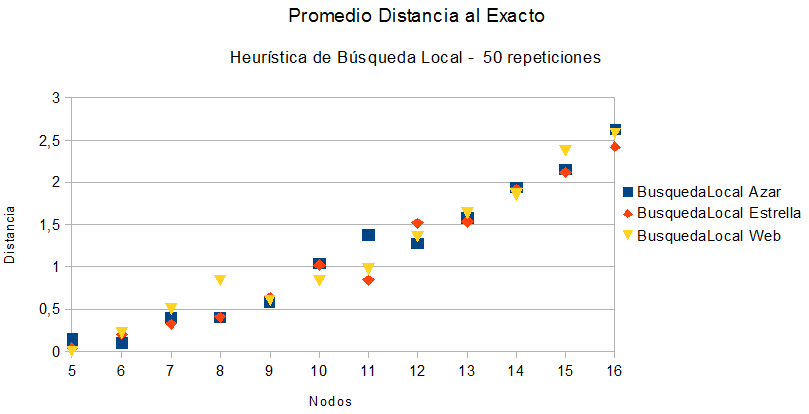
\includegraphics[scale=0.6]{distancia-BLocal.png}
\end{figure}

\quad Vemos un comportamiento menos estable que con el goloso con respecto a las distintas familias de grafos. Sin embargo la tendencia es clara, lineal. No se puede determinar una familia para el cual esta heurística es peor.

\begin{figure}[H]
	\centering
	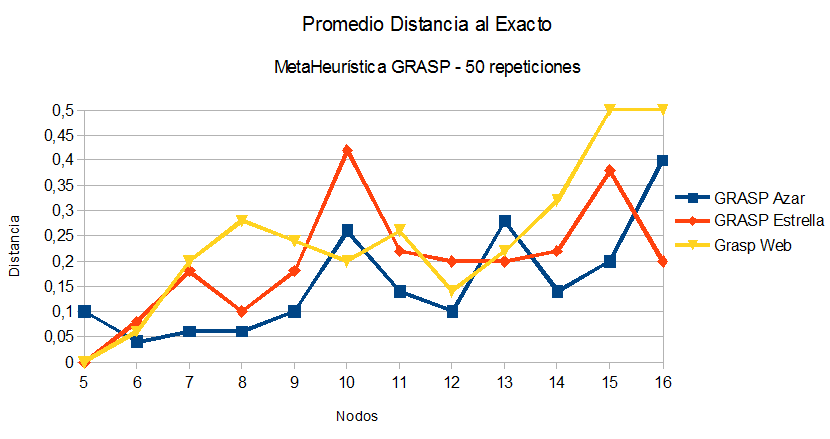
\includegraphics[scale=0.6]{distancia-GRASP.png}
\end{figure}

\quad Esta metaheurística es la menos estable de las 3. Varia mucho la distancia, presentando varios picos. Creemos que se debe a los criterios de parada definidos aunque hay que tener en cuenta que el promedio máximo es 0.5 menor a 1. Se podria decir que esta metaheuristica se comporta peor con las familias de grafo Web de 4 vertices porque con los grafos \textit{más grandes} es la que produce mayor distancia de la solución exacta.

\quad



\subsection{Comparando con Grasp}

\quad Dejando de lado el algoritmo exacto se puede experimentar con una mayor cantidad de nodos en un tiempo razonable.

\quad Comparamos entre si las heuristicas golosa, búsqueda local y GRASP.

\quad 

\subsubsection{Distancia}

\quad Vamos a calcular la distancia con el mismo criterio de la sección anterior, pero ahora tomando como punto de referencia la solución de la metaheurística GRASP.

\begin{figure}[H]
	\centering
	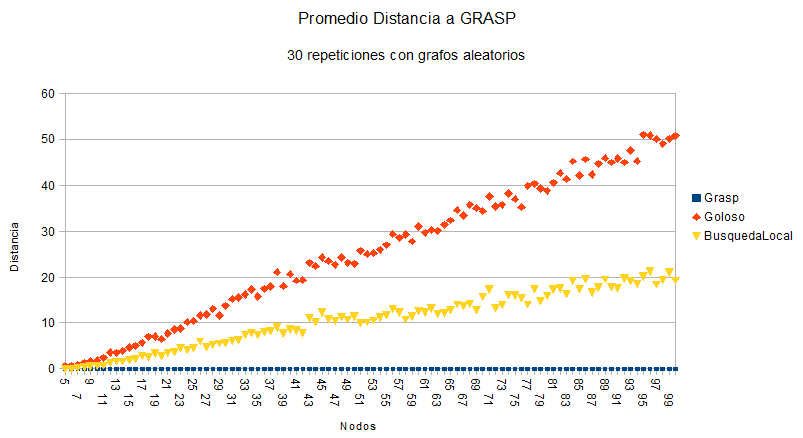
\includegraphics[scale=0.6]{distancia-Grasp-Azar.png}
\end{figure}

\begin{figure}[H]
	\centering
	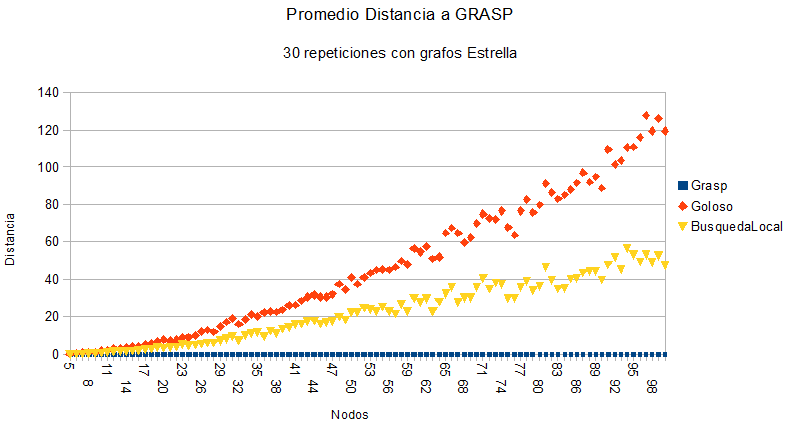
\includegraphics[scale=0.6]{distancia-Grasp-Star.png}
\end{figure}

\begin{figure}[H]
	\centering
	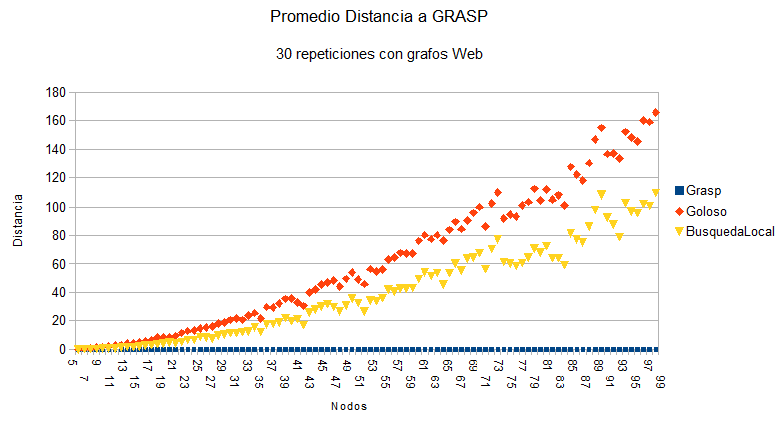
\includegraphics[scale=0.6]{distancia-Grasp-Web.png}
\end{figure}

\quad Se observa que en los grafos aleatorios la heurística constructiva golosa tiene un comportamiento lineal, en cambio en las otras familias es levemente exponencial.

\quad La heurística de búsqueda local tiene un comportamiento lineal con todas estas familias de grafos. Aunque en los grafos aleatorios es más uniforme, un poco menos estable en los grafos estrellas y mucho menos estable en los grafos Web de 4 vértices.

\quad Hay que tener en cuenta que usamos a GRASP como punto de referencia por lo que su distancia siempre es 0.

\quad Si nos fijamos en los valores obtenidos podemos ver como la calidad de las soluciones obtenidas empeoran pasando de una familia a otra. En este sentido las heuristicas golosa y de búsqueda local se comportaron igual. Donde mejor fue la calidad fue con la familia de grafos aleatorios. En un punto intermedio fue con los grafos estrella y donde peor calidad de solución se obtuvo fue en los grafos Web de 4 vértices.

\quad Estos resultados no se pudieron apreciar comparando con el método exacto debido a que no fue posible  poder experimentar con la misma cantidad de nodos ya que tomaria un tiempo no prudencial.

\subsubsection{Costo}

\quad Ahora analizaremos el costo temporal con las tres familias de grafos y comparando las heuristicas entre sí.

\begin{figure}[H]
	\centering
	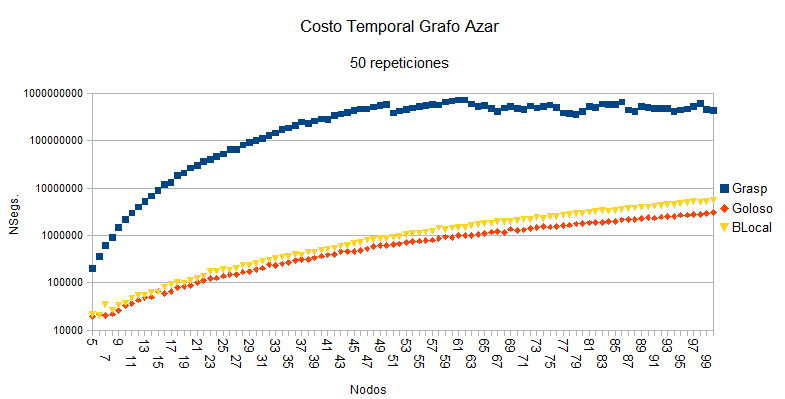
\includegraphics[scale=0.6]{timingAzar.png}
\end{figure}

\begin{figure}[H]
	\centering
	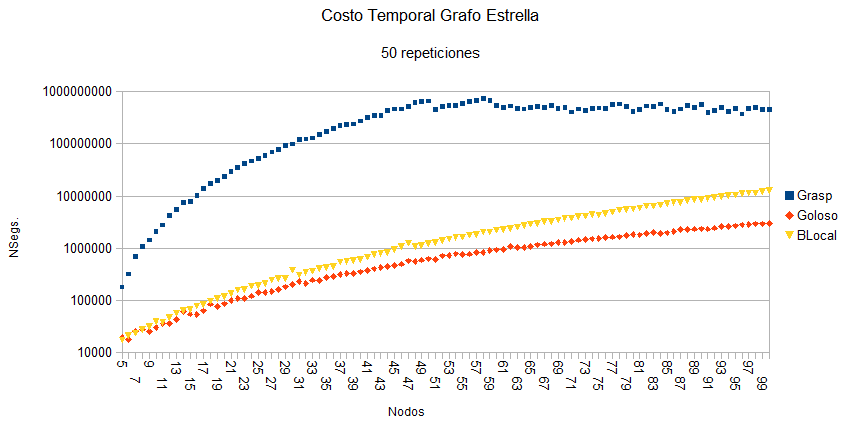
\includegraphics[scale=0.6]{timingStar.png}
\end{figure}

\begin{figure}[H]
	\centering
	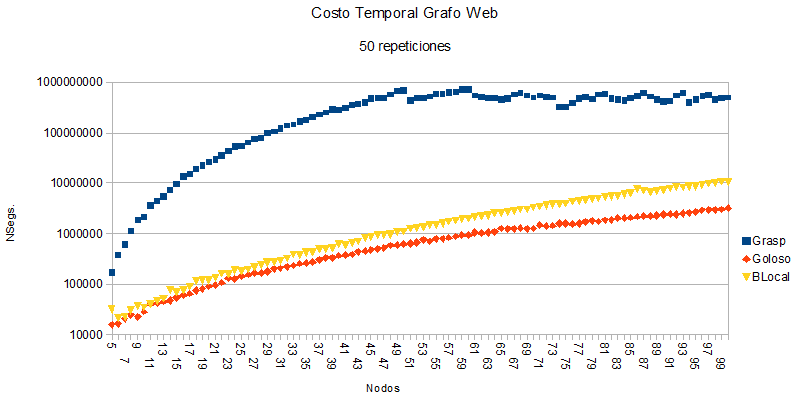
\includegraphics[scale=0.6]{timingWeb.png}
\end{figure}

\quad

\quad Debido a que GRASP arrojó resultados mucho mayores en comparación con las otras dos heurísticas, tuvimos que usar la escala logarítmica para poder compararlos mejor. Como era esperable teniendo en cuenta que usa los demás algoritmo al ejecutarse, los costos temporales de Grasp son mayores. Además, se aprecia que la Búsqueda Local cuesta un poco más que el goloso, algo que también era de suponerse al usar una solución golosa como semilla para encontrar una nueva solución.

\quad No se pueden apreciar diferencias relevantes entre los tres gráficos, por lo que deducimos que el tipo de familia del grafo no impacta demasiado en los costos.

\subsubsection{Conclusión Final}

\quad Como conclusión final, queda claro que ante la dificultad de ejecutar instancias con grafos muy grandes con el algoritmo exacto debido a su costo temporal, es conveniente hacer uso de alguna de las heurísticas detalladas durante este trabajo para aproximarnos a una solución aceptable. De las tres que implementamos la más costosa en complejidad es la metaheurística de Grasp (aunque con un costo muchísimo más pequeño que los costos para los casos análogos con el algoritmo exacto, por lo menos en aquellos dónde pudimos ejecutalo), pero sin embargo por la calidad de la solución que se obtiene usando este algoritmo consideramos que es preferible pagar el precio de una ejecución un poco más lenta, ya que si bien tanto la Búsqueda Local como el algoritmo goloso son más rápidos que Grasp, la calidad de la solución es bastante pobre si la comparamos con la que obtuvimos con el algoritmo exacto, cuando con Grasp se obtienen muy buenas aproximaciones a la solución exacta.

\quad Si se quitase Grasp de la ecuación y se tuviese que elegir entre la Búsqueda Local y el goloso, creemos conveniente hacer uso de la Búsqueda Local, ya que mejora la calidad de la solución golosa que se usa como semilla, costando un poco más temporalmente. Hay que recordar sin embargo que la solución obtenida con Búsqueda Local se trata de un máximo local, donde la localidad se define en base al concepto de vecindad que determinamos en el algoritmo.

